\documentclass[border=10pt]{standalone}

\usepackage{tikz}
\usepackage{tikzsymbols}
\usetikzlibrary{calc,patterns,shapes.geometric}

\def\centerarc[#1](#2)(#3:#4:#5){\draw[#1] ($(#2)+({#5*cos(#3)},{#5*sin(#3)})$) arc (#3:#4:#5);}

\begin{document}
	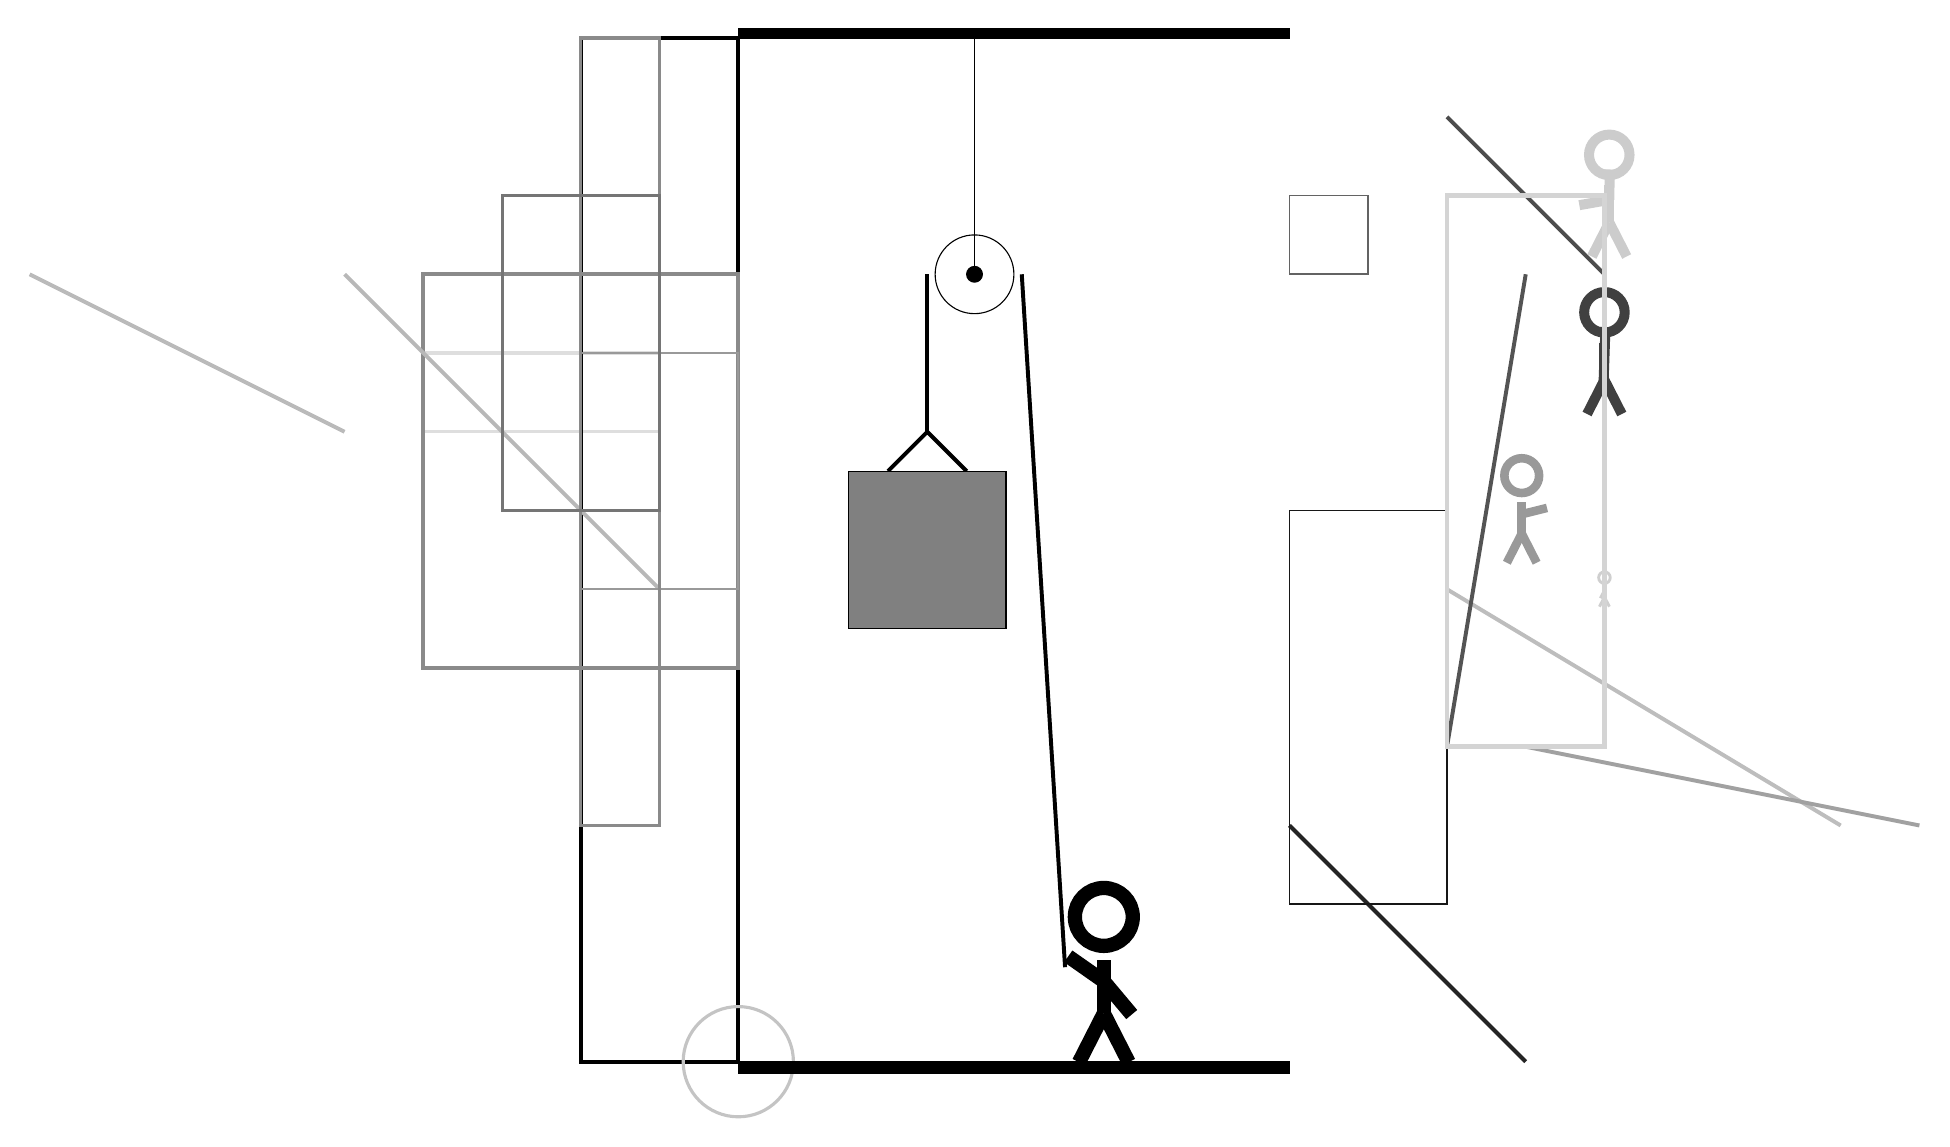
\begin{tikzpicture}
		%%%%% START %%%%%
		
		\draw[fill=black] (-2, 10) rectangle (5, 10.125);
		
		\draw (1, 7) circle (0.5);
		\draw[fill=black] (1, 7) circle (0.1);
		\draw (1, 10) -- (1, 7);
		
		\draw[line width=0.5mm] (-0.1, 4.5) -- (0.4, 5.0) -- (0.9, 4.5);
		\draw[fill=black!50] (-0.6, 4.5) rectangle (1.4, 2.5);
		
		\draw[line width=0.5mm] (0.4, 7) -- (0.4, 5.0);
		\centerarc[line width=0.5mm](1, 7)(0:180:0.6);
		\draw[line width=0.5mm](1.6, 7) -- (2.15, -1.8);
		
		\node at (2.6, -1.9) {\Strichmaxerl[10][-35][-50]};
		
		\draw[line width=0.4mm, color=black!13] (-3, 6) rectangle (-6, 5);
		
		\draw[line width=0.5mm, color=black!26](7, 3) -- (12, 0);
		\node[line width=0.6mm, color=black!40] at (8, 4) {\Strichmaxerl[6][90][14]};
		\draw[line width=0.5mm, color=black!100] (-2, 10) rectangle (-4, -3);
		
		\draw [line width=0.4mm, color=black!23](-2, -3) circle (0.7);
		\node[line width=0.4mm, color=black!19] at (9, 3) {\Strichmaxerl[2][62][80]};
		
		\draw[line width=0.2mm, color=black!99] (-2, -1) rectangle (-2, 0);
		\draw[line width=0.5mm, color=black!86](8, -3) -- (5, 0);
		\draw[line width=0.2mm, color=black!61] (5, 7) rectangle (6, 8);
		
		\draw[line width=0.5mm, color=black!67](7, 1) -- (8, 7);
		\draw[line width=0.5mm, color=black!46] (-2, 2) rectangle (-6, 7);
		\draw[line width=0.5mm, color=black!28](-3, 3) -- (-7, 7);
		\draw[line width=0.2mm, color=black!91] (5, 4) rectangle (7, -1);
		
		\draw[line width=0.3mm, color=black!40] (-4, 6) rectangle (-2, 3);
		\draw[line width=0.5mm, color=black!70](9, 7) -- (7, 9);
		\node[line width=0.6mm, color=black!75] at (9, 6) {\Strichmaxerl[7][88][88]};
		
		\draw[line width=0.4mm, color=black!46] (-4, 0) rectangle (-3, 10);
		\draw[line width=0.4mm, color=black!54] (-3, 8) rectangle (-5, 4);
		\draw[line width=0.5mm, color=black!37](8, 1) -- (13, 0);
		
		\draw[line width=0.5mm, color=black!27](-7, 5) -- (-11, 7);
		\node[line width=0.3mm, color=black!20] at (9, 8) {\Strichmaxerl[7][10][89]};
		\draw[line width=0.6mm, color=black!17] (7, 1) rectangle (9, 8);
		
		\draw[fill=black] (-2, -3) rectangle (5, -3.15);
		
		%%%%% END %%%%%
	\end{tikzpicture}
\end{document}